
\documentclass[journal, onecolumn, 11pt]{IEEEtran}
              
\usepackage{graphicx}
\usepackage{subcaption}
\usepackage{booktabs}
\usepackage{multirow}
\usepackage{hyperref}

\begin{document}

\title{Pilot: Momomood rhythms analysis}
\maketitle


\IEEEpeerreviewmaketitle

\section{Introduction}
Documentation for processing

\section{Methods}
Refer to main.tex for data processing procedure.

\section{Results}

\subsection{Statistics}


After applying the data availability criteria, 5 patients and 14 controls remained. In \autoref{tab:desc_events}, we present descriptive statistics of events data collected after the filtering process displayed above.


\begin{figure}[htbp]
  \centering
  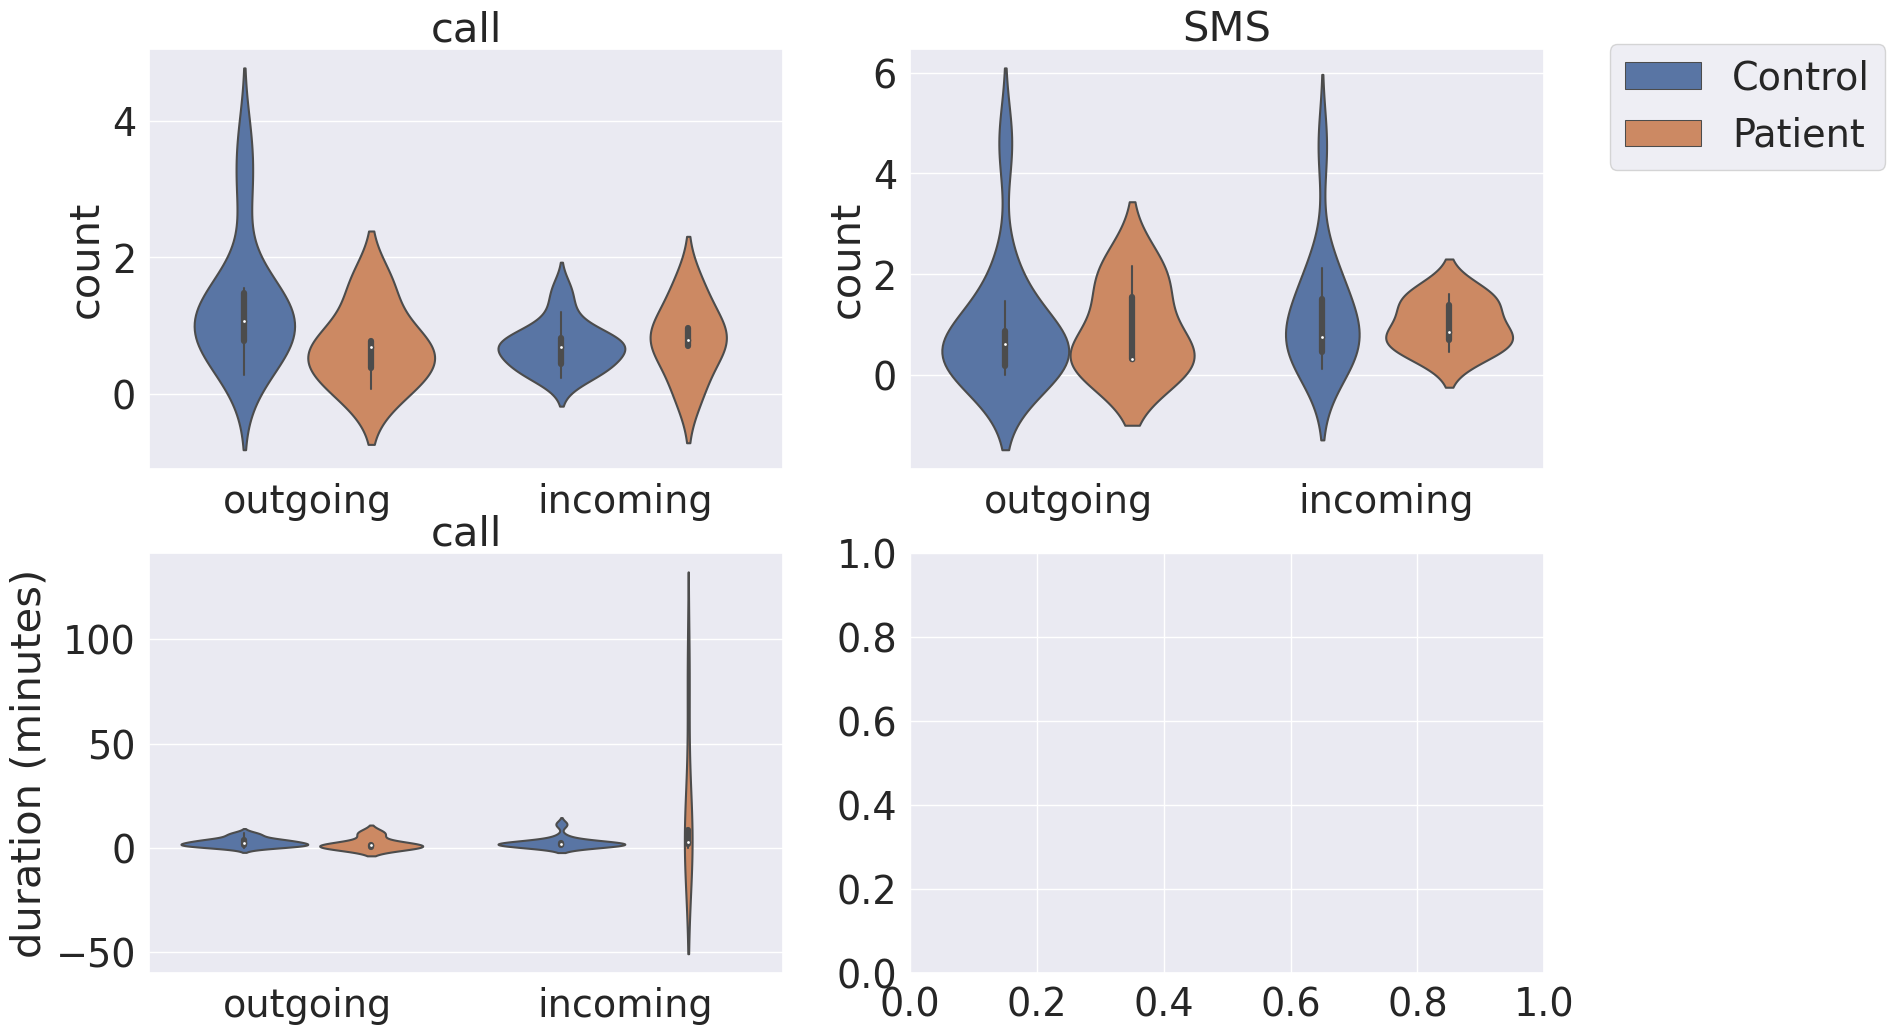
\includegraphics[width=\textwidth]{pilot_figs/1_pilot_descriptive_comm.png}
  \caption{Descriptive statistics of communications from pilot study}
\end{figure}

The result in incoming call duration was skewed by a user whose average incoming call was 81 minutes.

\subsection{Viz of daily/weekly rhythms}

\begin{figure}[hpt]
  \centering
  \begin{subfigure}[b]{0.75\textwidth}
    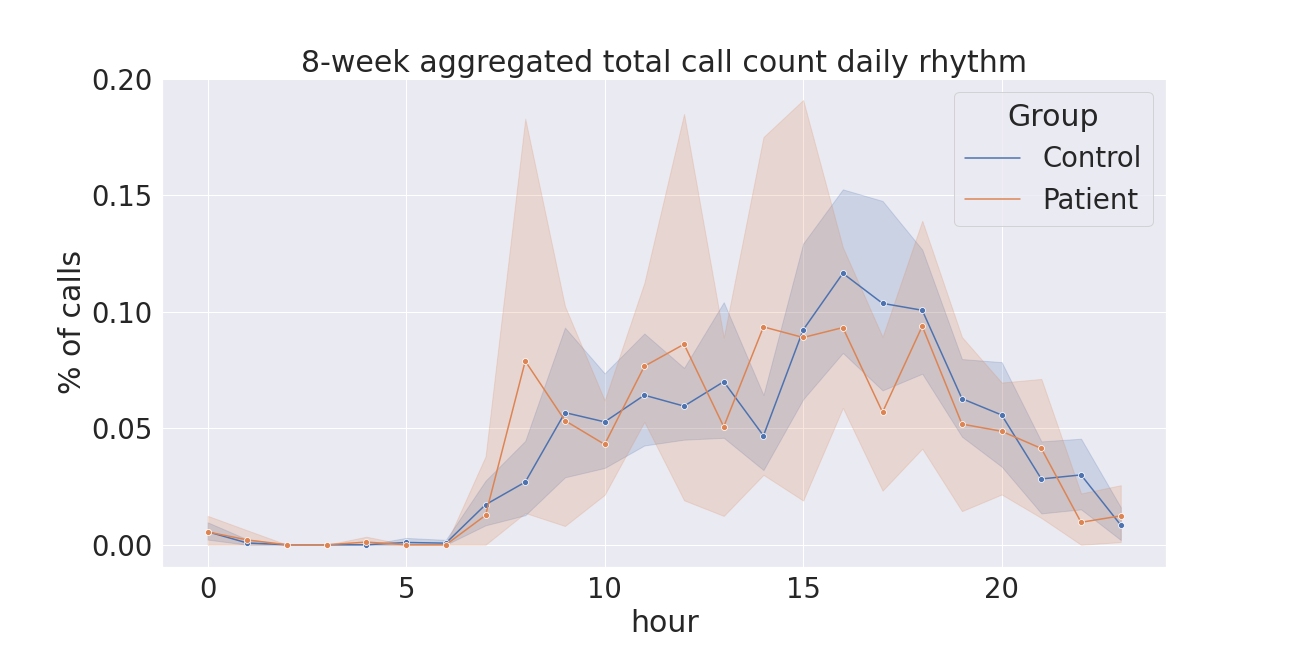
\includegraphics[width=\textwidth]{pilot_figs/agg_total_call_rhythm.png}
  \end{subfigure}

  \caption{Aggregated Daily and Weekly Rhythms.}
\end{figure}

\subsection{Calls}

\textbf{Inter-difference}

\subsection{Sleep}


\begin{figure}[hpt]
  \centering
  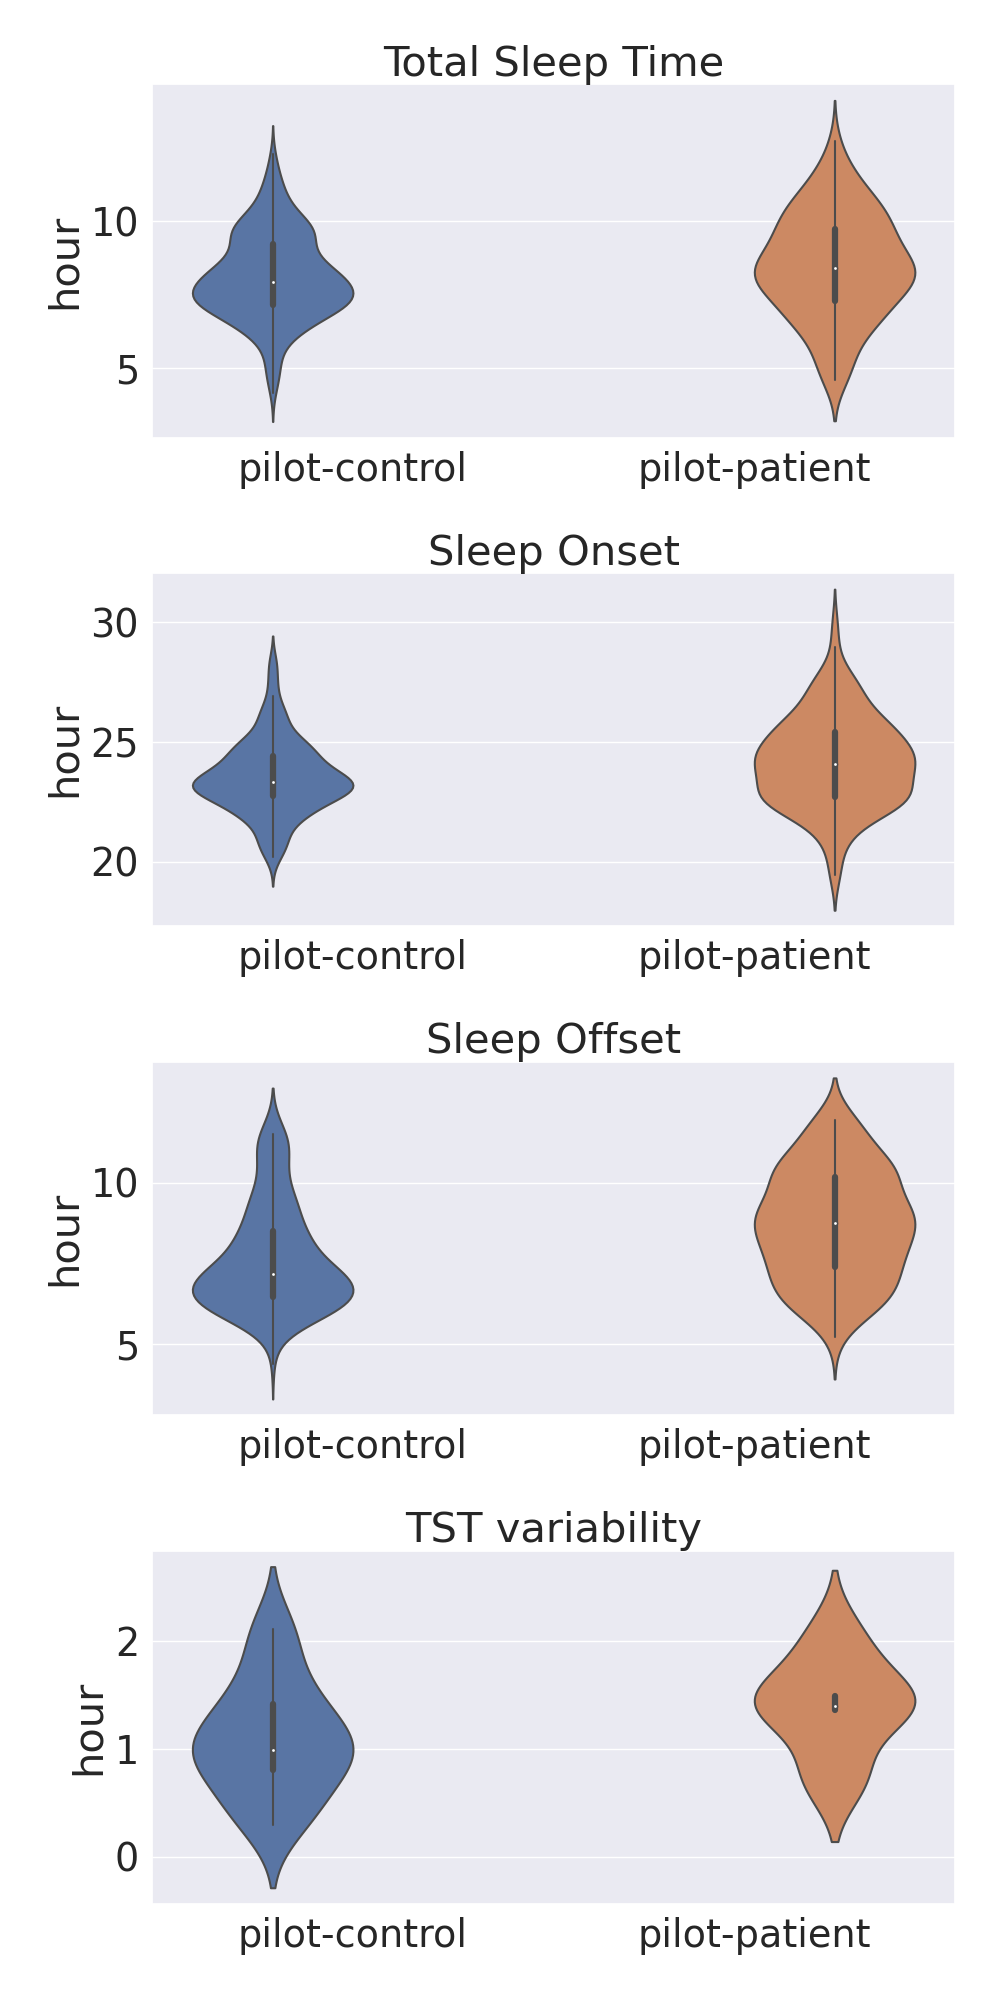
\includegraphics[width=0.7\textwidth]{pilot_figs/sleep_param.png}
  \caption{Sleep characteristics}
\end{figure}

Shapiro-Wilk test was performed to assess normality. TST variability was normally distributed, none of the other variables were normally distributed. T-test for TST var, MWU for the rest.

- Sleep onset and Sleep offset:. All results are significant: Patients go to bed later (p=0.001) and wake up later (p<0.001).

- TST: Result was significant. Patients sleep more than Control (p=0.04)

- TST variability: result was NOT significant (p=0.13).

\end{document}


\subsection{Occupation control}

\subsection{Outlier analysis}

\bibliographystyle{IEEEtran}
\bibliography{bibtex/blib}

\end{document}